\chapter{基于transformer和多尺度卷积的模型}
\label{cha:transformer}

为了更好地解决对某一目标的情感分析问题(Aspect-Term Sentiment Analysis, Target-oriented Sentiment Analysis),我们提出了使用transformer和多尺度卷积的模型。本章中,首先我们给出问题的形式化描述;然后,我们介绍transformer的结构;最后,介绍多尺度卷积的部分和目标函数。

\section{问题描述}

问题的输入是一个句子目标对$(w,w^\tau)$,其中目标$w^\tau=\{w^\tau_1,w\tau_2...w\tau_m\}$是句子$w=\{w_1,w_2...w_n\}$的子串,$m$是目标的长度,$n$是句子的长度。对某一目标的情感分析Aspect-Term Sentiment Analysis, Target-oriented Sentiment Analysis)的目标是提取句子所表达的对目标的情感极性$y\in \{P, N, O\}$,$P$,$N$,$O$分别表示积极、消极和中立。比如,句子“great food but the service was dreadful!”对目标“food”的情感极性是积极的,对目标“service”的情感极性是消极的。

\section{模型介绍}

\begin{figure}[ht]
    \centering  
    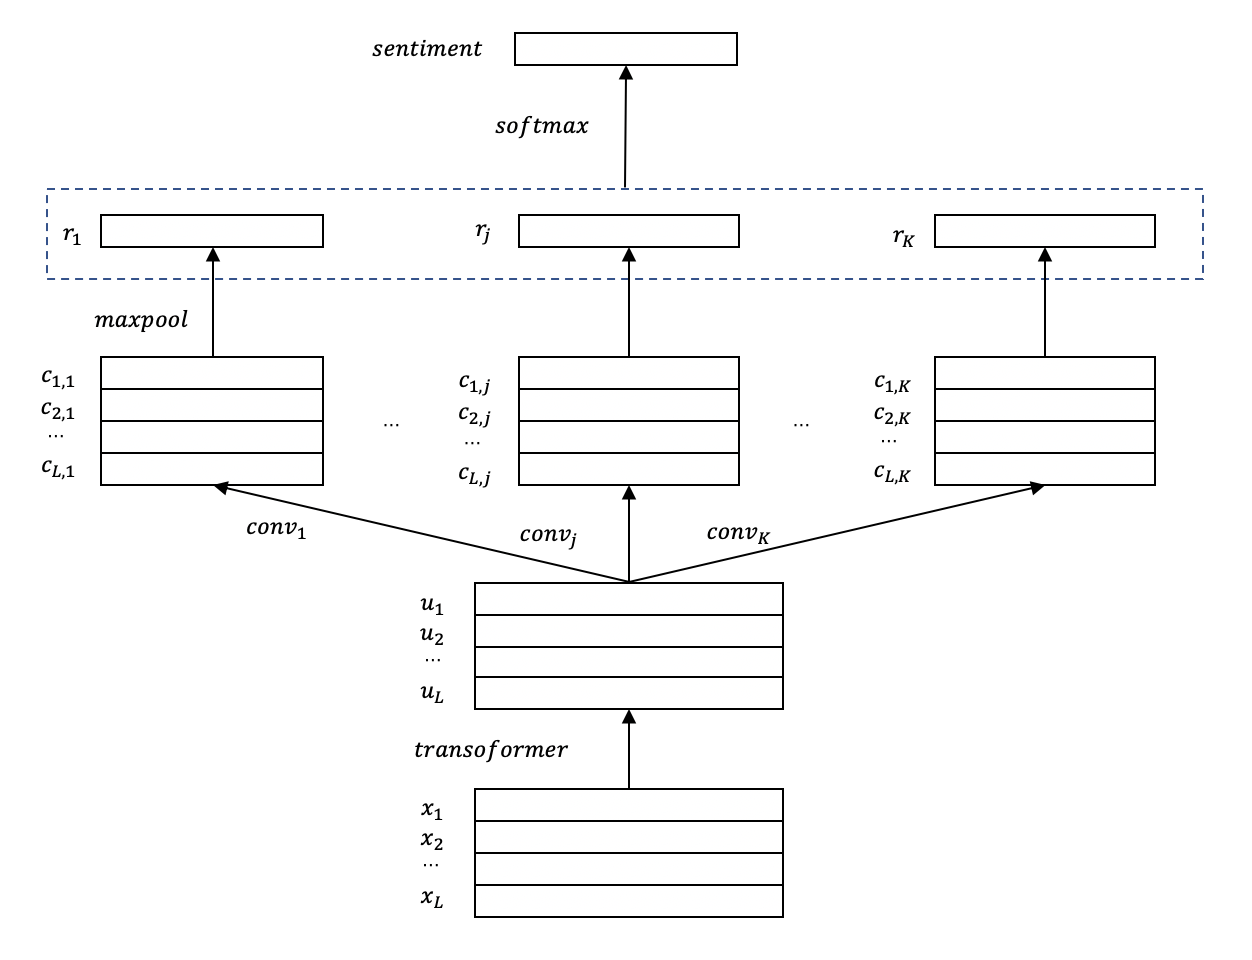
\includegraphics[width=0.8\linewidth]{transformer-model.jpg}
    \caption{基于transformer和多尺度卷积的模型}
    \label{fig:transformer-model}
\end{figure}

图~\ref{fig:transformer-model}显示了我们所提出的模型的主要结构。我们将目标和句子拼接起来,并用多层transformer结构来处理;多尺度卷积可以学习变长n-gram特征。

\section{Transformer结构}

循环网络结构RNN和卷积神经网络CNN经常被用来将一个变长序列映射成一个固定长度的序列。循环网络结构RNN一般沿着序列的时间维度,逐个地生成隐层状态。循环网络RNN天然地具有时序性,这也使得循环网络结构在训练过程中难以被并行。当序列长度较长时,RNN往往难以训练。

卷积神经网络CNN通过局部感受野,获取输入序列的局部特征。但是,由于卷积的局部性,导致单层卷积难以学习长期的依赖关系;多层卷积可以弥补这一问题,但长期依赖的路径变长。

Transformer~\cite{NIPS2017_7181}不依赖循环网络结构和卷积神经网络,只通过self-attention就将输入序列映射到固定长度的输出序列。在本小节中,我们将简要地介绍transformer的结构。

\begin{figure}[ht]
    \centering 
    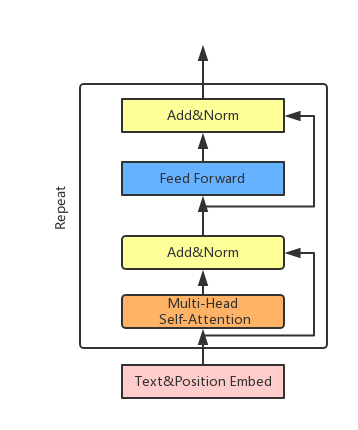
\includegraphics[width=0.5\linewidth]{transformer.jpg}
    \caption{Transformer结构}
    \label{fig:transformer}
\end{figure}

图~\ref{fig:transformer}显示了transfomer的结构。Transformer是一个多层结构,每一层包括self-attention和前向网络。

\subsection{点积attention}

点积attention与常见的attention机制不同,它的Attention权重是由点积求得的。对于query~$Q\in R^{T_q\times d_k}$,key $K\in R^{T_v\times d_k}$和value$V\in R^{T_v\times d_v}$,attention的输出是
\begin{equation}
    Attention(Q,K,V)=softmax(\frac{QK^T}{\sqrt{d_k}})V
\end{equation}
其中,$T_q$是query的长度,$T_v$是key和value的长度,$d_k$是query和key的维度,$d_v$是value的维度。$\sqrt{d_k}$用来地权值进行缩放,保证了权值的稳定性。
\subsection{多头attention}
Transformer中并没有使用单一的attention机制,而是用不同的线性映射将query,key,value映射$h$次。多次attention机制可以看作是单一attention的一种ensemble模型。多个映射将query,key,value映射到了不同的子空间,多头attention侧重于不同的值。
\begin{equation}
    \begin{aligned}
        MultiHead(Q,K,V)&=concat(head_1,head_2...head_h)W^O\\
        head_i&=Attention(QW^Q_i,KW^K_i,VW^V_i)
    \end{aligned}
\end{equation}
其中用到的映射都是不包含偏置的线性映射,其中$W^Q_i\in R^{d_{model}\times d_k}$,$W^K_i\in R^{d_{model}\times d_k}$,$W^V_i\in R^{d_{model}\times d_v}$是需要学习的参数,$d_{model}$是单词向量的维度。
Self-attention是$Q$、$K$、$V$相同的多头attention。
\begin{equation}
    SelfAttention(V)=MultiHead(V,V,V)
\end{equation}
\subsection{前向网络}
在transformer的每一层中,除了用到了attention机制,还使用了一个两层全连接网络,使用relu激活函数。
\begin{equation}
    FFN(x)=relu(xW_1+b_1)W_2+b_2
\end{equation}
\subsection{词向量和softmax}
与其他序列模型类似,我们将输入单词和输出单词映射为一个需要学习的向量,向量的维度是$d_{model}$。模型的最后,使用一个带有softmax激活函数的线性层得到预测结果。
\subsection{位置编码}
因为多头attention机制和前向网络没有卷积层和循环结构,不能处理输入序列的时序信息,我们使用了位置编码来弥补这一缺点。这里用到的位置编码是在训练过程中学习得到的,而不是利用提前定义好的\cite{radford2018improving}。
\section{语言模型和预训练}

在本小节,我们都语言模型和使用transformer的语言模型做简要的介绍。一个统计语言模型通常构建为句子$w$的概率分布$P(w)$,这里$P(w)$实际上反映的是$w$作为一个句子出现的概率。对于一个由$n$个词按顺序构成的句子$w=\{w_1,w_2...w_n\}$,$P(w)$实际上求解的是字符串的联合概率,利用贝叶斯公式,链式分解如下:
\begin{equation}
    P(w)=P(w_1,w_2...w_n)=P(w_1)P(w_2|w_1)P(w_3|w_1,w_2)...P(w_n|w_1,w_2...w_{n-1})
\end{equation}
从上面可以看出,语言模型可以看成,在给定了前一个词的情况下,求下一个词出现的条件概率。在这里,我们使用的是基于transformer的语言模型。设$W_e$是词向量表示,$W_p$是位置编码,$h_l$表示第$l$层的中间结果。初始句子表示为
\begin{equation}
    h_0=UW_e+W_p
\end{equation}
我们用$transformer\_block$表示transfomer的每一层。
\begin{equation}
    h_l=transformer\_block(h_{l-1})
\end{equation}
则最终的概率分布为
\begin{equation}
    P(w)=softmax(h_nW^T_e)
\end{equation}
语言模型的训练只需要句子本身,因此其训练数据非常的充足。之前的研究表明,使用在大规模语料库上预训练的语言模型的参数,可以大大提升分类任务的效果。我们使用OpenAI GPT\cite{radford2018improving}提供的预训练的语言模型,将语言模型的输出用作特征。OpenAI GPT是在BooksCorpus数据集上训练的,它包括七千本未发表的书籍,内容包括了冒险、奇幻、史诗类作品。另一个数据集是1B
Word Benchmark\cite{Zhu2015Aligning},它与BookCorpus有类似的大小。在这个语料库上训练该语言模型,直到达到了18.4的困惑度(perplexity)。我们用预训练得到的参数去初始化transformer的参数,之后在对某一目标的情感分析任务中去调优这些参数。

本小节中使用的符号是为了解释语言模型的相关问题,与其他章节的符号无关,并不冲突。
\section{多尺度卷积}
我们把对某一目标的情感分析问题( Aspect-Term Sentiment Analysis, Target-oriented Sentiment Analysis)转化为一个序列对分类问题。具体地,我们把句子$w=\{w_1,w_2...w_n\}$和目标$w^\tau=\{w^\tau_1,w^\tau_2...w^\tau_m\}$拼接起来,在开头添加一个$start$记号,在结尾添加一个$end$记号,并在句子和目标之间添加一个$del$记号。拼接得到的序列记为$X$,$X=\{start,w_1,w_2...w_n,del,w^\tau_1,w^\tau_2...w^\tau_m,end\}=\{x_1,x_2...x_L\}$,其中$L=m+n+3$。将$X$输入到一个多层transformer结构当中,得到每个单词的表示。在这里,为了简洁,我们用下面的方式表示多层transformer结构。
\begin{equation}
    u_1,u_2...u_L=transformer(x_1,x_2...x_L)t
\end{equation}
一般情况下,$start$记号的表示$u_1$被用来当作整个输入的表示。这种方式忽略了其它单词的表示,而这些信息可能会对预测正确的情感极性有着重要的作用。为了解决这一问题,我们使用多尺度的卷积来处理所有单词的表示。在句子中,有许多不同长度的短语。多尺度的卷积可以提取不同长度短语的特征。我们使用了多个不同卷积核大小的卷积层,并在序列的两端补零使不同卷积的输出大小保持一致。$K$是卷积的数量。
\begin{equation}
    c_{i,j}=tanh(u_{i:i+k_j}*W_j+b_j)
\end{equation}
其中,$W_j$和$b_j$是第$j$个卷积的参数,$k_j$是第$j$个卷积核的大小。我们使用max pooling层来选取最重要的特征。
\begin{equation}
    r_j=max(c_{1,j},c_{2,j}...c_{L,j})
\end{equation}
把max pooling的输出结果拼接起来,得到句子的最终表示。
\begin{equation}
    r=concat(r_1,r_2...r_K)
\end{equation}
最后,使用带有softmax激活函数和全连接层得到预测结果。
\begin{equation}
    \hat{y}=softmax(Wr+b)
\end{equation}
其中$W$和$b$是全连接层的参数。
\section{目标函数}
训练过程中,我们的目标是最小化损失函数,损失函数是语言模型的损失函数和分类损失函数的和。
\begin{equation}
    Loss=Loss_{lm}+Loss_{clf}
\end{equation}   
语言模型的损失函数为
\begin{equation}
    Loss_{lm}=\sum_{i}\sum_{n}\hat{x_{i,n}}log(x_{i,n})
\end{equation}
其中,$x_i$是语言模型的第$i$个输出,$n$是单词的序号。分类损失函数是真实值$y$和预测值$\hat{y}$的交叉熵。
\begin{equation}
    Loss_{clf}=\sum_{i}\sum
    _{j}\hat{y_{i,j}}log(y_{i,j})
\end{equation}
其中,$i$是样本的序号,$j$是输出类别的序号。
